\documentclass{article}
\usepackage{blindtext}
\usepackage[a4paper, total={6in, 9.4in}]{geometry}
\usepackage{indentfirst}
\usepackage{wrapfig}
\usepackage{graphicx}
\usepackage{mathtext}
\usepackage{amsmath}
\usepackage{siunitx} % Required for alignment
\usepackage{subfigure}
\usepackage{multirow}
\usepackage{rotating}
\usepackage{afterpage}
\usepackage[T1,T2A]{fontenc}
\usepackage[russian]{babel}
\usepackage{caption}
\usepackage[arrowdel]{physics}
\usepackage{booktabs}

\graphicspath{{pictures/}}

\title{\begin{center}Лабораторная работа №4.1.1\end{center}
Метод Аббе}
\author{Севастьян Черняков и Иван Юдин}
\date{\today}

\begin{document}

\pagenumbering{gobble}
\maketitle
\pagenumbering{arabic}

  \maketitle

\textbf{Цель работы:} определение дифракционного предела разрешения объектива микроскопа методом Аббе.



\section{Экспериментальная установка}
  Схема модели проекционного микроскопа приведена на рис. Предметом служат сетки, расположенные в кассете. Смена сеток осуществляется поворотом внешнего кольца кассеты.
  % \begin{figure}[H]
  %   \center{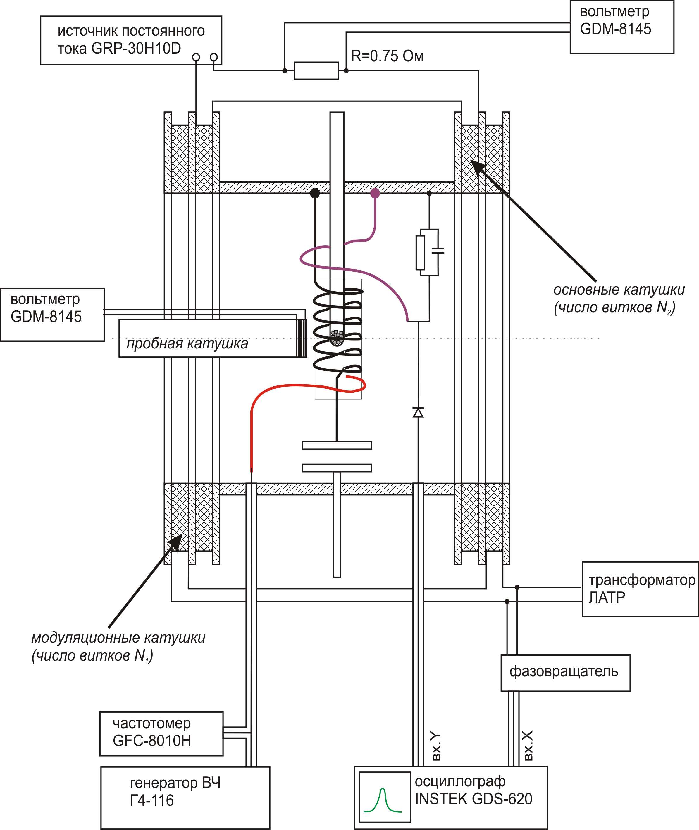
\includegraphics[scale=1.0]{ustanovka.pdf}}
  %   \caption{Схема экспериментальной установки -- модель проекционного микроскопа.}
  %   \label{ris:ustanovka}
  % \end{figure}
  Изображение сетки периодически повторяется -- \textit{репродуцируется} -- в пространстве между сеткой и первой линзой. Для выделения геометрического изображения среди множества репродуцированных изображений сетки на одну из сеток наложена эмблема физтеха, то есть непереодический объект, изображение которого не репродуцируется.
  
\section{Ход работы}
  \begin{enumerate}
    \item
      Определение периода решёток по их пространственному спектру
    \item 
      Определение периода решёток по изображению, увеличенному с помощью модели микроскопа
    \item
      Определение периодов решёток по оценке разрешающей способности микроскопа
    \item 
      Наблюдение явлений пространственной фильтрации и мультиплицирования.
  \end{enumerate}
\newpage
\section{Экспериментальные данные}

  Измерим расстояние $L = 1200$ мм от сетки до экрана и определим периоды решёток по их пространственному спектру. Для этого выразим $d = m \lambda / \sin \theta$, причем $\sin \theta \approx (l/n)/L$ и $m = 1$, где $l$ -- расстояние между удалёнными друг от друга максимумами. Используемый нами лазер имеет длину волны $\lambda = 532$ нм.
  
\begin{table}[]
\centering
\begin{tabular}{|c|c|c|c|}
\hline
№ Сетки & x, мм & y, мм & d, мкм             \\ \hline
1       & 66,3  & 66,3  & $9,73\pm 0,13$     \\ \hline
2       & 26,7  & 26,7  & $24,49 \pm 0,84$   \\ \hline
3       & 13,3  & 13,3  & $ 50,73 \pm 3,62 $ \\ \hline
\end{tabular}
\end{table}
  
  Определим периоды решёток по изображению, увеличенному с помощью микроскопа по формуле $d = (l/n)/\Gamma$, где $\Gamma = \frac{b_1b_2}{a_1a_2}$ -- увеличение для оптической системы.

 
% \begin{table}[H]
% \centering
% \begin{tabular}{|c|c|c|c|c|c|c|}
% \hline
% № Сетки & a_1, мм & a_2, мм & b_1, мм & b_2, мм & $d_{\text{'}}$ & d, мкм             \\ \hline
% 1       & 125     & 70      & 755     & 300     & 0,75           & $9,42\pm 0,73$     \\ \hline
% 2       & 125     & 130     & 380     & 420     & 2              & $27,43 \pm 1,08$   \\ \hline
% 3       & 125     & 130     & 130     & 480     & 5              & $ 56,69 \pm 2,29 $ \\ \hline
% \end{tabular}
% \end{table}


\begin{table}[h]
  \begin{center}
  \begin{tabular}{|c|c|}
  \hline
   № кольца &  r, мм \\
  \hline
   1 & 16 \\  \hline
   2 & 26 \\ \hline
   3 & 38 \\ \hline
   4 & 46 \\ \hline
   5 & 54 \\ \hline
   6 & 60 \\ \hline
  
  
   
  \end{tabular}

  Определим для каждой решётки минимальный размер диафрагмы $D$, при котором на экране ещё видно изображение двумерной сетки. По формуле $d =~2\lambda f_1 / D$. $f_1 = 110$ мм


  % \begin{table}[H]
  %   \centering
  %   \begin{tabular}{|c|c|c|}
  %   \hline
  %   № Сетки & D, мм           & d, мм        \\ \hline
  %   1       & ~--             & ~--          \\ \hline
  %   2       & $ 3,8 \pm 0,1 $ & $28 \pm 1 $  \\ \hline
  %   3       & $ 1,7 \pm 0,1 $ & $ 63 \pm 2 $ \\ \hline
  %   \end{tabular}
  %   \end{table}
    
      
    
        
    
    
      
      
      
      
      % \begin{figure}[H]
      %   \center{\includegraphics[scale=0.6]{433.jpg}}
      %   \caption{Зависимость $d=d\,(1/D)$.}
        
      % \end{figure}
    
    
    \section {Обсуждение результатов}
      В ходе данной лабораторной работы мы определили периоды дифракционных решёток различными способами. Полученные результаты отличаются друг от друга несущественно, хотя и не попадают в ворота погрешностей друг-друга. Это может быть связано с приближенным характером используемой теории, неточностью определения величин $a_2$ и $b_1$, нечёткостью перехода от двумерной сетки к одномерной. 
      
      
      Не смотря на расхождения, нам удалось убедиться в справедливости формулы $2\lambda f \approx d D $, т.к. $2\lambda f = 117$ мм $\cdot$ мкм, а коэффициент наклона графика $k = 107$ мм $\cdot$ мкм, т.е. проверка теории Аббе оказалась положительной. 
      
    
    \section{Качественные наблюдения}
    
        При достаточно маленькой толщине щели, на экране видно полоски, каждый раз параллельные направлению щели.
    
        Эффект мультиплицирования изображения также был получен.
      
    
    
\end{document}
    